% !TEX root = paper.tex

\documentclass[11pt,letterpaper]{article}

% Packages
\usepackage{packages}
\addbibresource{sources.bib}

% Document Settings
\geometry{margin=1in}
\setlength{\parskip}{1ex}
\setlength{\parindent}{0pt}

\pagestyle{fancy}
\lhead{Väinö-verneri Kauppila} % controls the left corner of the header
\chead{} % controls the center of the header
\rhead{} % controls the right corner of the header
\lfoot{} % controls the left corner of the footer
\cfoot{} % controls the center of the footer
\rfoot{Page~\thepage} % controls the right corner of the footer
\renewcommand{\headrulewidth}{0.4pt}
\renewcommand{\footrulewidth}{0.4pt}

% =========================================
%             DOCUMENT
% =========================================

\begin{document}
%\doublespacing % Double spacing throughout the document


% =========================
%      TITLE PAGE
% =========================

% Suppresses headers, footers, and page numbers on title page
\begin{titlepage}
    \begin{center}
        \vspace*{4cm}
        Geography\\
        Internal Assessment \\
        \vspace{1cm}
        How does environmental quality, determined by the severity of pollution and the availability of green spaces, differ between a tourist-catering area of Paris versus a residential area? \\
        \vspace{1cm}
        \textit{Väinö-verneri Kauppila} \\
        May 2021 \\
        \vspace{4cm}
        Word count: TBD \\
        \vfill
        \vspace{0.1cm}
    \end{center}
\end{titlepage}

% =========================
%      DOCUMENT BODY
% =========================

\pagenumbering{roman}

\begin{center}
    \pdfbookmark{\contentsname}{Contents}
    \tableofcontents
    \vspace{1in}

\end{center}


% TODO: Add hyper-references to links
% TODO: Improve listings' styling
% TODO: Add links to Contents entries

\newpage

\pagenumbering{arabic}

\section{Introduction}




\subsection{Hypotheses}

\begin{enumerate}
    \item According to the Global Development Goals of the UN, 90\% of urban areas in the world had polluted air in 2016. \footcite{sdg_report_2020} Paris was among these countries that didn't satisfy WHO's air quality minimum \footcite{ambient_outdoor_air_pollution_2018} of 2018, with on average a 50\% higher than normal pollution density. In addition, the areas of tourism in Paris are, as seen in Figure 1, higher in pollution than residential areas. However, a counterargument to this could be that despite a higher concentration of people, tourist areas in Paris do not suffer as much from high traffic conditions from things such as typical morning rush hours, and tourists preferably using public transport or bikes.

    \item 2nd hypothesis
    \item 3rd hypothesis
\end{enumerate}


\begin{figure}[h!]
    \centering
    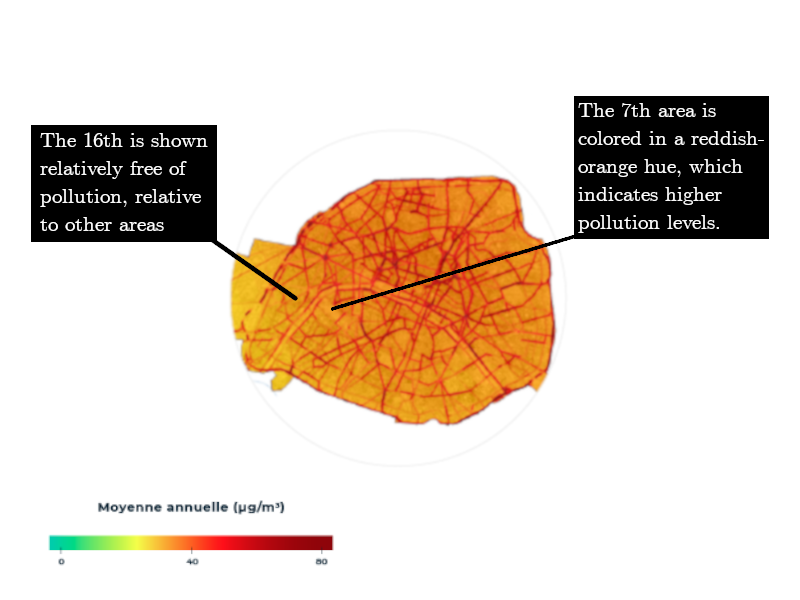
\includegraphics[width=0.7\linewidth]{no2_map.png}
    \caption{A map of Paris NO2 levels in 2018, as reported by AirParif, on the official Paris website \footcite{paris_air_qual}}
\end{figure}



\section{Method}


For our investigation, the topic in question is the environmental quality. We shall compare the environmental quality of two areas, one meant as a residential one and one with a heavy tourist presence. To best represent these areas, we have chosen the XVIe and the VIIe, justifiable as the XVIe is home to many housing complexes and fosters facilities aimed at catering to the residents whereas the VIIe sees many tourists as it is home to the famed Eiffel Tower and the Seine river, prime tourist attractions of Paris.



\subsection{Sampling choices}

The method we will be using to select the sites from where we will take the Bipolar survey is Stratified which means that we are choosing the sites ourselves. The reason we chose this is to make sure that we got a good variety of sites that would give a good idea of the general environmental quality of that area, but also to avoid the selection of residential areas, which do in fact exist in the VIIe, which would happen if we chose the random sampling method. This stratified sampling approach would best represent the targeted area and yield meaningful data on tourist-heavy sites.

The sampling method we used to select our sites is the stratified method. The reason for this choice is that we get a

\subsection{Study site choices}

To best retrieve data from our sites, we shall maintain a fair test to uphold the standard and quality of our reliability by getting our data at around the same time on the same day of the week, in an attempt to best match up with the tourists’ habits. We have chosen the time frame of 14:00 to 16:00 on a Friday afternoon, a time frame where tourists will not be constrained by lunch or sleep.

\section{Analysis}

Lorem

\subsection{Environmental and cultural sustainability}
Lorem ipsum dolor sit amet

\subsection{Economic sustainability}
Lorem ipsum dolor sit amet

\section{Conclusion}

Lorem ipsum dolor si amet

\newpage
\pagenumbering{roman}


\section*{Notes}
\label{sec:notes}
\addcontentsline{toc}{section}{\nameref{sec:notes}}

This paper is written with the aid of the typesetting software \LaTeX. On a PDF viewer, the sections in the table of contents can be clicked to access that section.

\printbibliography

\appendix
\section{Appendix}
\label{app}

\subsection{Appendix Test}
\label{app:test}


\end{document}